	\subsection*{Pre- und In-Game Adaption}
		\subsubsection{Atari Puffer, CatEye Video Game Bike}\label{ergometer}
			Die einfachste Art der Pre- und In-Game Adaption bieten Exergaminggeräte. Exemplarisch hierfür 						\textit{Atari Puffer} und das \textit{Video Game Bike} der Firma \textit{CatEye}.
			\\ \\
			Der 1982 von Atari entwickelte \textit{Atari Puffer} (Abb \ref{ataripuffer}) \cite{Sinclair:2007:CDE:1321261.1321313} war das erste System, welches die Möglichkeit bieten
			sollte Videospiele mit dem Körper zu steuern. Plan war es eine Art Fahrradergometer an den \textit{Atari} 					anzuschließen um somit die Spiele zu steuern. Eine erhöhte Umdrehungszahl der Pedale sollte dafür sorgen,
			dass zum Beispiel das Auto des Spielers im Spiel \textit{Pole Position}\footnote{\url{http://www.atarimania.com/game-atari-2600-vcs-pole-position_8020.html}} schneller fuhr oder der Spieler im Spiel
			\textit{Dig-Dug}\footnote{\url{http://www.8-bitcentral.com/reviews/2600digDug.html}} schneller gräbt. Zusätzlich konnte ein Gamepad am Lenker montiert werden um zusätzliche
			Eingaben zu ermöglichen.
			\\ \\
			\textit{Atari} plante drei verschiedene Versionen seines \textit{Puffers}:
			\begin{itemize}
				\item{Pro Model, mit eingebautem Pulsmessgerät, für Fitnessstudios}
				\item{Arcade Model, für Spielhallen}
				\item{Home Model, für den Privathaushalt. Geplanter Preis: 140-170\$}
			\end{itemize}
			Auf Grund der Videospielkrise im Jahr 1984 kam es jedoch nie zur Markteinführung.
			\\ \\
			\begin{figure}[h]
 				\centering
   	 			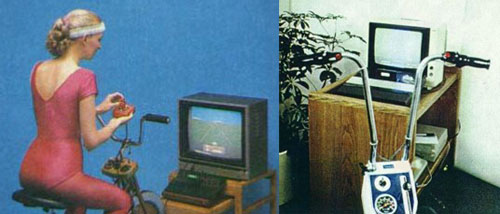
\includegraphics[width=7cm]{gfx/ataripuffer.jpg} 
    				\caption{Atari Puffer}
   	 			\label{ataripuffer}
			\end{figure}
			\\ \\
			Ein ähnliches System bietet \textit{CatEye} (Abb \ref{gamebike}) mit dem \textit{Video Game Bike}. Hierbei 				handelt es sich ebenfalls um ein Fahrradergometer. Es kann sowohl mit den Videospielkonsolen von \textit{Sony} (\textit{Playstation 1 \& 2})\footnote{\url{http://de.playstation.com/}} als auch \textit{Nintendo}\footnote{\url{http://www.nintendo.de/}} und \textit{Xbox}\footnote{\url{http://www.xbox.com/de-DE}} betrieben werden und funktioniert mit sämtlichen Spielen, die auf Geschwindigkeit basieren.
			\\ \\
			 Im Handel sind zwei Versionen erhältlich:
			\begin{itemize}
				\item{CatEye Game Bike Home Model GB-200, für 399\$}
				\item{Game Bike Pro, 1449\$, für den kommerziellen Gebrauch}
			\end{itemize}
			Der Adaptionsmechanismus, den diese Geräte bieten, lässt sich sowohl vor, als auch während des Spielens 					nutzen. Hierzu wird der mechanische Widerstand am jeweiligen Gerät erhöht, beziehungsweise verringert. Diese Anpassung muss aber jeweils manuell erfolgen. Die Geräte bieten keine Möglichkeit automatisch den Widerstand zu erhöhen. 
%--------------------------------------------------------------------------------------------------------------------------------------------------
		\subsubsection{Thera Trainer}\label{theravital}
			\label{theratrainer}
			Die Firma \textit{medica Medizintechnik GmbH}\footnote{\url{http://www.thera-trainer.de/}} entwickelt, neben dem \textit{Balance-Trainer}, verschiedene Geräte und Programme zur Unterstützung der Bewegungstherapie. Mögliche Anwendungszwecke sind beispielsweise die Therapie von Schlaganfällen, sowie von Muskel- und rheumatischen Erkrankungen. Es findet jedoch auch Anwendung auf dem Gebiet der Orthopädie und Kardiologie. Hierzu bietet der Hersteller verschiedene Trainingsgeräte in Form von Ergometern und Balance Plattformen. Im folgenden wird das \textit{Thera-vital} System betrachtet.
			\\ \\
			Einige Eigenschaften des Ergometers:
			\begin{itemize}
				\item{Drehzahl, Drehrichtung, Widerstand, Therapiezeit einstellbar}
				\item{Aktives/Passives Training}
				\item{200 Watt Motor}
				\item{Trainingsauswertung}
				\item{...}
			\end{itemize}
\begin{figure}[htbp]
	 	 		\centering
	  			\begin{minipage}[b]{6 cm}
    					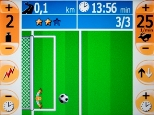
\includegraphics{gfx/Torwart.jpg}
    					\caption{Torwart}
    					\label{Torwart}
	  			\end{minipage}
  				\begin{minipage}[b]{6 cm}
    					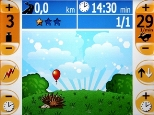
\includegraphics{gfx/Igel.jpg}
    					\caption{Igel}
    					\label{Igel}
  				\end{minipage}
				\begin{minipage}[b]{6 cm}
    					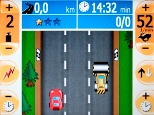
\includegraphics{gfx/Auto.jpg}  
    					\caption{Auto}
    					\label{Auto}
  				\end{minipage}
				\begin{minipage}[b]{6 cm}
    					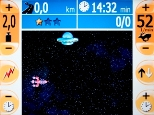
\includegraphics{gfx/Planet.jpg}  
    					\caption{Planet}
    					\label{Planet}
  				\end{minipage}
			\end{figure}
			Durch die Möglichkeit Ziel-Drehzahl, Widerstand und Therapiezeit einzustellen wird ein manueller mechanischer 				Pre-, beziehungsweise In-Game Adaptionsmechanismus bereitgestellt.
			Je nach gesundheitlicher Beinträchtigung kann das Ergometer mit den Armen oder den Beinen bedient 					werden. Auf dem am Gerät montierten Bildschirm können vier verschiedene optische Feedbacksysteme 					angezeigt werden:
			\\ \\
			\textbf{Torwart:}\\
				Der Patient bewegt den Fußballtorwart durch Erhöhung und Reduzierung der Drehzahl nach oben und unten 					um möglichst viele Torschüsse abzuwehren. (Abb \ref{Torwart})
			\\ \\
			\textbf{Igel:} \\
				Durch unterschiedliche Kraftverteilung des linken und rechten Beins bewegt sich der Igel in die 						entsprechende Richtung. Herabfallende Gegenstände sollen dadurch zum platzen gebracht werden. 					(Abb \ref{Igel})
			\\ \\
			\textbf{Auto:}\\
				Der Patient sieht eine Fahrbahn, sowie sein eigenes Fahrzeug. Ziel ist es möglichst viele andere 						Fahrzeuge zu überholen. Hierzu muss er schneller Treten als eine voreingestellte Drehzahl. Durch 						Veränderung der Kraftverteilung (siehe \textit{Igel}) kann das Auto nach links und rechts bewegt werden. (Abb \ref{Auto})
			\\ \\
			\textbf{Planet:}\\
				Der Patient muss mit seinem Raumschiff Planeten nach oben und unten ausweichen. Dabei kann 						zwischen konzentrischem und exzentrischem Training gewählt werden. Beim konzentrischen Training 					muss eine gewisse Kraft erbracht werden um das Raumschiff zu bewegen. Beim exzentrischen muss 					die Kraft hingegen abgebremst werden. (Abb \ref{Planet})
\\ \\			
			Der Austausch der Assets ist bei den jeweiligen Spielen nicht möglich. Allerdings kann man die Bereitstellung 				dieser vier verschiedener Mini-Spiele als eine Möglichkeit betrachten die Spiellogik zu verändern.
%------------------------------------------------------------------------------------------------------------------------------------------------
		\subsubsection{Jeff Sinclaire - Edith Cowan University}
			Bei dem Exergaming Projekt der \textit{Edith Cowan University Perth} \cite{5716909} handelt es sich um einen einfachen Side-Scroller, der mit einem Fahrradergometer gesteuert wird (Abb \ref{sidescroller}). Ziel des Spiels ist es einen 						Hubschrauber in der richtigen Höhe zu halten und dabei Gegenstände einzusammeln, Hindernissen 						auszuweichen und Gegner abzuschießen. 
			\\ \\
			Als Ergometer kommt hierbei das \textit{GameBike} der Firma \textit{CatEye} (Abb \ref{gamebike}) zum Einsatz. Das 					Ergometer kann an die gängigsten, auf dem Markt erhältlichen Spielekonsolen angeschlossen werden und funktioniert mit sämtlichen Spielen, die auf Geschwindigkeit basieren. Für das Projekt der Universität Perth wurde eine Modifikation vorgenommen um es auch an einen PC anschließen zu können.
			\begin{figure}[h]
  				\centering
  				\begin{minipage}[b]{6 cm}
   	 				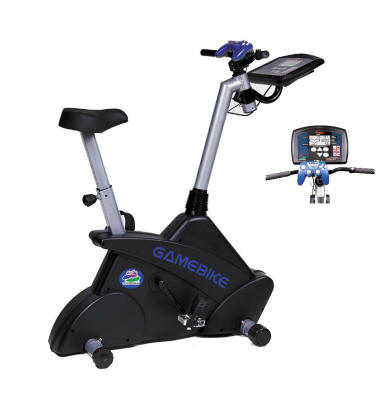
\includegraphics[width=6cm]{gfx/cateye.jpg} 
    					\caption{CatEye GameBike}
    					\label{gamebike}
  				\end{minipage}
				\begin{minipage}[b]{6 cm}
    					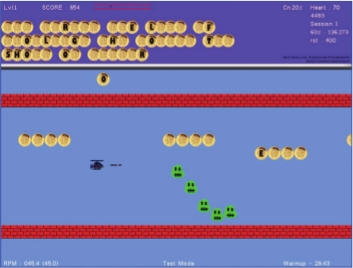
\includegraphics[width=6cm]{gfx/edith.jpg}  
    					\caption{Side Scroller}
    					\label{sidescroller}
  				\end{minipage}
			\end{figure}
\\
			Je schneller der Spieler tritt, desto höher fliegt der Helikopter. Verringert der Spiele die Geschwindigkeit 					verliert der Helikopter an Höhe. Das Spiel bietet mehrere Adaptionsmöglichkeiten. Einerseits ist eine Erhöhung 				des Tretwiderstandes vor und während des Spielens am Ergometer möglich, zum anderen können vor dem 					Starten des Spiels Anpassungen im Spiel vorgenommen werden, die zur Adaption beitragen. Beispiele hierfür 				sind Platzierung und Anzahl der Bonusgegenstände, der Gegner, sowie die Trittfrequenz, die nötig ist um den 				Helikopter in einer bestimmten Höhe zu halten. Eine Veränderung der Spiellogik, sowie der Assets ist nicht 					möglich.
%------------------------------------------------------------------------------------------------------------------------------------------------
		\subsubsection{Ergo Active}\label{ergoactive}
			Entwickelt wurde \textit{Ergo Active} an der \textit{Technischen Universität Darmstadt} \cite{Gobel:2010:SGH:1873951.1874316} zur Förderung von Serious Games for Health mit wissenschaftlichem Hintergrund, in Bezug auf Sport und Gesundheit. Es umfasst drei Spiele \textit{Taubenjagd, Film} und \textit{Balance} zum Ausdauer-, beziehungsweise Herz-Kreislauftraining. Gesteuert werden alle drei Spiele mittels eines Fahrradergometers.
			\\ \\
			\textbf{Taubenjagd:} \\
Hierbei handelt es sich um einen einfachen Sidescroller. Der Spieler steuert eine 	Brieftaube mit Hilfe des Fahrradergometers. Ziel ist es vorbei fliegende Briefe einzusammeln um Punkte zu bekommen. Um so schneller er tritt, desto höher fliegt die Taube. Der Spieler tritt dabei innerhalb eines vorher festgelegten Geschwindigkeit Intervalls, wodurch einerseits verhindert wird, dass der jeweilige Spieler ausserhalb seiner körperlichen Möglichkeiten trainiert und andererseits ein Adaptionsmechanismus für verschiedene Spieler gegeben ist. 
			\\ \\
			\textbf{Film:} \\
\textit{Film} ermöglicht dem Spieler zum Beispiel Etappen der \textit{Tour de France nachzufahren}. Hierfür wird ein Film der jeweiligen Strecke gezeigt. Je nach dem wie schnell der Spieler Tritt um so schneller wird der Film der jeweiligen Etappe abgespielt. Ähnlich wie bei Taubenjagd findet auch hier eine Überwachung des Spielers statt. Über-, oder unterschreitet er seine Leistungsgrenzen gibt das Spiel ein Signal um den Spieler daraufhin zuweisen wieder innerhalb seines persönlichen Intervalls zu trainieren.
			\\ \\
			\textbf{Balance:} \\
Bei \textit{Balance} hat der Spieler zwei Aufgaben. Er balanciert einen Clown auf einem Ball. Hierzu muss er mittels Ergometer eine vorgegebene Geschwindigkeit halten, beziehungsweise darf maximal nur um einen bestimmten Wert davon abweichen. Während er den Clown in der Balance hält fallen Luftballons herab, die er mittels Maus oder Wiimote\footnote{\url{http://www.nintendo.com/wii/what-is-wii/\#/controls}} abschießen muss, um Punkte zu sammeln. Die voreingestellte Geschwindikeit und die maximale Abweichung dienen hierbei zur Überwachung, damit  sich der Spieler innerhalb seiner Leistungsgrenzen bewegt. 
			\begin{figure}[h]
	  			\centering
  				\begin{minipage}[b]{6 cm}
    					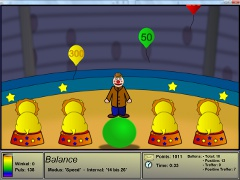
\includegraphics[width=6cm]{gfx/balance.jpg} 
    					\caption{Ergo Active - Balance}
    					\label{balance}
  				\end{minipage}
				\begin{minipage}[b]{6 cm}
    					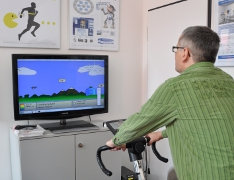
\includegraphics[width=6cm]{gfx/ergoactive.jpg} 
    					\caption{Taubenjagd}
    					\label{ergoactive}
  				\end{minipage}
			\end{figure}
\\
	 		"Film" bietet durch Austausch der Videos gleichzeitig eine, wenn auch sehr geringe, Veränderung der Assets. 				Bei \textit{Taubenjagd} und \textit{Balance} ist kein Assettausch möglich. Ähnlich wie bei den Spielen des 				\textit{Thera Trainers} (Kap \ref{theratrainer}) findet ein vergleichbarer Effekt wie bei Veränderung der Spiellogik durch die verschiedenen Spiele statt.
			\\ \\
			Die Adaption findet zweigeteilt statt. In der ersten Phase wird vor dem Spiel die Individuelle Leistungsfähigkeit 				eingestellt (vgl. \ref{wissenschaft}). Die zweite Phase findet während dem Spielen statt. Über die 						Rückmeldungen der Vitalparameter kann das Spiel auf verschiedene Situationen reagieren. So kann zum Beispiel 			über ein Pulsmessgerät am Ohrläppchen auf eine zu hohe Herzfrequenz reagieren und den Widerstand am 				Ergometer automatisch herabsetzen.
			\\ \\
			Alle drei Spiele sind in der Programmiersprache \textit{Java} implementiert. \textit{Taubenjagd} und 				\textit{Balance} bilden die Grundlage für die in dieser Arbeit realisierten Spiele. Hierzu werden sie von Java in 				die Spieleentwicklungsumgebung \textit{Unity3D} (siehe \ref{unity}) portiert und erweitert.
